% !TeX program = pdflatex
% !BIB program = biber
%
% From News Text to Causal Infographics via Semantic Triplets
% Final numbers (n=10) from experiments/seminar_triplets/evaluation/aggregate_scores.py.

\documentclass[sigconf,natbib=false, language=english]{acmart}

\usepackage[datamodel=acmdatamodel, style=acmnumeric, backend=biber, sorting=none]{biblatex}
\DefineBibliographyStrings{english}{nodate = {}}

\usepackage{graphicx}
\usepackage{booktabs}
\usepackage{xcolor}
\usepackage{listings}
\lstdefinestyle{snip}{basicstyle=\ttfamily\scriptsize, breaklines=true,
  numbers=none, frame=single, framesep=4pt, xleftmargin=2pt, aboveskip=4pt, belowskip=2pt,
  backgroundcolor=\color{black!3}}
\lstset{style=snip}
\usepackage{tikz}
\usetikzlibrary{arrows.meta, positioning, fit, backgrounds}
\usepackage{subcaption}
\addbibresource{refs.bib}
\usepackage{csquotes}

\AtBeginDocument{%
  \providecommand\BibTeX{{%
    \normalfont B\kern-0.5em{\scshape i\kern-0.25em b}\kern-0.8em\TeX}}}

\setcopyright{rightsretained}
\copyrightyear{2026}
\acmDOI{}
\acmConference[SiKDD 2026]{Slovenian KDD Conference 2026}{October 2026}{Ljubljana, Slovenia}
\acmISBN{}
\settopmatter{printccs=false, printacmref=false}
\geometry{a4paper}

\begin{document}

\title[From News Text to Causal Infographics via Semantic Triplets]{From News Text to Causal Infographics via Semantic Triplets: Making an Opaque Image Pipeline Inspectable}

\author{Georgi Trajkov}
\email{geotrajkov0@gmail.com}
\affiliation{%
  \institution{Jožef Stefan Institute}
  \city{Ljubljana}
  \country{Slovenia}
}

\begin{abstract}
The MedVrsticami/BetweenTheLines news-analysis system renders an event's coverage as a single causal-network infographic, generated end-to-end by a text-to-image model. This is convenient but opaque: the knowledge graph the picture depicts exists only inside the model, so it cannot be inspected, corrected, or verified. We study what happens when an explicit \emph{semantic triplet} (subject--predicate--object) stage is inserted between the article text and the image, applied to the production MedVrsticami/BetweenTheLines pipeline. We compare two conditions on the same Slovene events---direct generation and a triplet-mediated image (both rendered by the same model)---under a two-layer rubric that separates triplet correctness from rendered-image faithfulness. Across ten events we find that decomposition does \emph{not} yield a better infographic: the direct image is somewhat more faithful and clearer, and $2.3\times$ denser, though the triplet image matches or beats it on faithfulness in half the events. The triplet stage's value is elsewhere: it makes the pipeline \emph{auditable}. We measure that extraction is $\sim$70\% clean while the image model mis-draws $\sim$19\% of the edges of an otherwise-correct graph (mostly wrong connections)---a failure that is invisible and unattributable in the black-box baseline. This separates the pipeline's two error sources, and the explicit intermediate opens downstream possibilities---selective rendering, cross-event linking via shared triplets, and connecting nodes to per-publisher sentiment---that an end-to-end model forecloses.
\end{abstract}

\keywords{Semantic Triplets, RDF, Knowledge Graphs, Large Language Models, Text-to-Image, News Analysis, Causal Infographics, Pipeline Transparency}

\maketitle

\section{Introduction}
Platforms such as Event Registry~\cite{leban2014event,eventregistry} and Ground News~\cite{groundnews} aggregate news around events and expose bias and sentiment indicators. Building on Event Registry, the MedVrsticami/BetweenTheLines system~\cite{betweenthelines} performs fine-grained cross-source analysis of how individual claims and entities are portrayed by different publishers. One of its outputs is a \emph{causal-network infographic}: a single editorial-quality image, generated directly from the articles by a text-to-image model (Gemini~3 Pro Image Preview), that lays out the actors and events of a story as a node--link diagram.

The infographic is produced in one step: article text in, picture out. The graph it depicts---which entities are nodes, which causal relations are edges, in which direction---is never materialized. It lives only inside the image model. This makes the artifact impossible to inspect, query, correct, or evaluate except by eye, and any error (a reversed arrow, an invented link, a dropped relation) is indistinguishable from a deliberate editorial choice.

We ask a simple question: \emph{what does inserting an explicit, inspectable knowledge-graph stage between text and image buy us, and at what cost?} We add a semantic triplet extraction step---subject--predicate--object relations with stable entity identifiers, mirroring RDF~\cite{rdf11}---and feed the resulting graph to the renderer instead of raw text. This echoes the task-decomposition principle that made BetweenTheLines's claim classification accurate: decompose the task, expose the intermediate, evaluate each stage.

Our contributions are: (1) a triplet schema and extraction prompt that produces connected, source-grounded causal graphs at the density of real infographics, with confidence and source-language constraints; (2) a controlled two-condition comparison (direct vs.\ triplet-mediated image) under a two-layer rubric that separates \emph{triplet correctness} from \emph{rendered-image faithfulness} on the same events; and (3) the finding that, for this pipeline, the decomposition's value is transparency and fault-localization rather than image quality---it separates the two error sources the black box conflates, localizing the largest avoidable failure to the generative rendering step.

\section{Related Work}
\textbf{Cross-source news analysis.} Ground News~\cite{groundnews_harford,groundnews_wvu} classifies publishers on a left--right spectrum and aggregates coverage, but does not track individual claims or produce structured graphs. Event Registry~\cite{leban2014event,eventregistry} clusters articles into events and provides article-level VADER sentiment~\cite{hutto2014vader}. BetweenTheLines~\cite{betweenthelines} builds on Event Registry with multi-prompt LLM analysis of entity and claim portrayal; the causal infographic studied here is one of its presentation layers.

\textbf{Relations and graphs from text.} Extracting structured relations from natural language is the classic domain of Open Information Extraction~\cite{banko2007openie,fader2011reverb}, which produces subject--relation--object tuples without a fixed schema. More recently, LLMs have largely taken over knowledge-graph and triplet construction~\cite{bian2025kgsurvey}, and have been applied specifically to extracting \emph{causal} graphs from text in a zero-shot fashion~\cite{antonucci2024causal}, where LLM-derived priors are found especially useful for \emph{orienting} edges~\cite{darvariu2024priors}---a step our results show the image renderer often gets wrong. Our triplets are an LLM-produced, schema-light variant, but our aim differs: we extract the causal graph in order to \emph{render} it as an infographic---and to measure how faithfully a downstream image model redraws it---rather than to populate a database. The entities map naturally to RDF subjects/objects and the predicates to RDF properties~\cite{rdf11}, which is what makes the intermediate queryable and standardizable in principle.

\textbf{Text-to-image for diagrams.} General text-to-image models render legible editorial graphics but offer no guarantee of structural fidelity to a specified graph. A central question of this paper is precisely how faithfully such a model reproduces a supplied node--link structure.

\section{The Current Infographic Pipeline}
For an event, the production step (\texttt{CausalNetworkInfographicService}) concatenates the \emph{title and body of every article in the event cluster} (capped at the ten most relevant articles) into one text block, and sends it to Gemini~3 Pro Image with a single prompt that asks the model to both \emph{extract} a causal knowledge graph and \emph{render} it as a Bloomberg/Economist-style node--link infographic (Listing~\ref{lst:prod}). The two responsibilities---deciding the graph and drawing it---are fused in one opaque call. The output is a raster image; no node list, edge list, or evidence is emitted. There is therefore no way to ask which relations the picture claims, whether they are supported by the articles, or whether the drawing even matches the model's own intended graph.

\begin{lstlisting}[caption={Excerpt of the production prompt: a single call both extracts and renders the graph from the concatenated articles.}, label={lst:prod}]
### Content Processing Rules
Analyze the provided text to extract a Knowledge Graph:
* Nodes: key Entities and Key Claims/Events.
* Links: Causal Relations connecting these nodes.
* Logic: visual flow represents the chain (Cause -> Effect).
### Input Text
{articles}   # title + body of every article in the event
\end{lstlisting}

\section{Proposed Method}
We insert an explicit triplet stage and render from it (Figure~\ref{fig:pipeline}).

\textbf{Triplet schema.} Extraction returns a JSON object with an \texttt{entities} list (stable \texttt{id}, human-readable \texttt{label}, one \texttt{central} flag) and a \texttt{triplets} list (\texttt{subject\_id}, \texttt{predicate}, \texttt{object\_id}, \texttt{evidence} span, \texttt{confidence}). Because subjects and objects reference entity \texttt{id}s, reuse across triplets is structural, not lexical---the graph is connected by construction. The \texttt{entities} map to RDF subjects/objects and \texttt{predicate} to a (currently free-text) property~\cite{rdf11}.

\textbf{Extraction prompt.} Calibrated against real production infographics (12--18 nodes, 6--10 distinct entities), the prompt targets 10--15 triplets over 6--10 entities and enforces: a single connected component with no singleton entities; specific predicates (banning generic ``affects/relates to''); a strict \emph{source-language lock} (labels, predicates, and evidence stay in the article language); \emph{event reification} (a death, ruling, or attack becomes its own node rather than collapsing onto a person); and \emph{attribution-in-predicate} for contested claims (e.g.\ \emph{naj bi} / ``allegedly (per the defense)''), so a one-sided allegation is not stated as fact. A validator checks connectivity and id consistency and retries once on failure.

\textbf{Confidence filtering.} Each triplet carries low/medium/high confidence; low-confidence triplets are filtered before rendering. In our data the model's own ``low'' flag tended to mark mis-grounded triplets, letting them be dropped automatically---a controllability lever the black-box pipeline cannot offer.

\textbf{Two rendering paths (evaluated).} (1) \emph{Direct}: the unchanged baseline, text$\rightarrow$image. (2) \emph{Triplet$\rightarrow$image}: the same image model and visual-style prompt, but fed the explicit entity and edge lists instead of raw text. Both use Gemini~3 Pro Image~\cite{gemini}, so the only difference is the input.

Because the triplets are now explicit, they could also be rendered \emph{programmatically} (e.g.\ a deterministic \texttt{graphviz} layout~\cite{graphviz}), which would reproduce the graph with perfect structural fidelity. Producing a result as readable and information-dense as the generative image, however, requires a typed node ontology and an icon/visual-encoding library (flags, currency, institutional symbols)---substantial design work that is out of scope here. We therefore evaluate only the two generative conditions and treat programmatic rendering as a direction enabled by, but not delivered in, this study.

\begin{figure}[t]
  \centering
  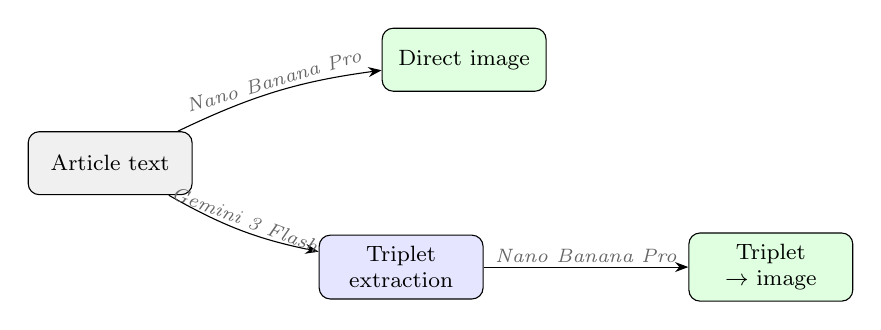
\begin{tikzpicture}[
    >=Stealth,
    box/.style={draw, rounded corners, align=center, inner sep=4pt,
                minimum height=8mm, text width=18mm, font=\footnotesize},
    art/.style={box, fill=gray!12},
    gen/.style={box, fill=blue!10},
    rbox/.style={box, fill=green!12},
    elab/.style={font=\scriptsize\itshape, text=black!60, sloped, above, midway, inner sep=1.5pt}]
    \node[art] (text) {Article text};
    \node[rbox, above right=5mm and 24mm of text] (direct) {Direct image};
    \node[gen, below right=5mm and 16mm of text] (trip) {Triplet extraction};
    \node[rbox, right=26mm of trip] (ti) {Triplet $\rightarrow$ image};
    \draw[->] (text) to[bend left=9] node[elab]{Nano Banana Pro} (direct);
    \draw[->] (text) to[bend right=9] node[elab]{Gemini 3 Flash} (trip);
    \draw[->] (trip) -- node[elab]{Nano Banana Pro} (ti);
  \end{tikzpicture}
  \caption{The two evaluated conditions and the model at each stage. The direct baseline fuses extraction and rendering in one opaque call; the triplet condition exposes the graph, then renders it. Extraction uses Gemini~3 Flash; both image renders use Gemini~3 Pro Image (\emph{Nano Banana Pro}).}
  \label{fig:pipeline}
\end{figure}

\section{Evaluation Design}
\textbf{Data.} Ten Event Registry events, each with 5--10 Slovene-language articles (mean 9.0 articles/event, mean article body $\approx$1{,}570 characters; Table~\ref{tab:dataset}). Article bodies are truncated to 3{,}000 characters in the enriched prompt.

\textbf{Models.} Extraction uses \texttt{gemini-3-flash-preview} (temperature 0.2, JSON mode, article bodies capped at 3{,}000 chars). \emph{Both} image conditions use \texttt{gemini-3-pro-image-preview} (\emph{Nano Banana Pro}) at 2K, 16:9, with \emph{identical} settings---the only difference is the input (raw text vs.\ supplied triplets), which is what makes the head-to-head fair.

\textbf{Rubric (two layers).} A single rater scores each event. \emph{Layer 1---the final image} (same basis for both pipelines, judged against the articles): faithfulness (1--5) and relation clarity (1--5), plus a by-eye node count for density. \emph{Layer 2---the triplet stage} (inspectable, so partly objective): a per-triplet verdict on a severity scale (correct~/ \emph{minor}: misleading, awkward, imprecise~/ \emph{error}: wrong direction, wrong predicate, wrong endpoints, unsupported, redundant), event-level coverage (1--5), and---for triplet$\rightarrow$image---a per-edge render verdict (drawn correctly, wrong direction, wrong connection, omitted) checked against the known graph, plus a count of unsupported additions.

\textbf{Decontamination.} The few-shot examples in the extraction prompt were rewritten to a fictional scenario so that none of the ten evaluation events appear in the prompt, removing train-on-test leakage; provenance of every prompt revision is retained.

\section{Results}
Ten events, single rater; 115 triplets and 114 rendered edges scored.

\textbf{The triplet image is competitive but does not win (Table~\ref{tab:image}).} The direct image is modestly more faithful ($4.10$ vs.\ $3.10$, mean difference $1.0$) and clearer ($3.60$ vs.\ $2.80$), but the gap is not decisive: the triplet$\rightarrow$image matches or beats the direct image on faithfulness in $5$ of $10$ events. The one robust direct advantage is density: $18.4$ vs.\ $8.0$ nodes, a $2.3\times$ gap. This gap is structural---the direct image freely promotes quantities, dates, and outcomes to nodes, whereas the triplet schema admits only typed entities.

\textbf{Extraction is mostly sound but not error-free (Table~\ref{tab:codebook}).} Of 115 rated triplets, 69.6\% are correct and 25.2\% have only minor issues (chiefly \emph{imprecise} or \emph{misleading} phrasing); 5.2\% are hard errors, dominated by \emph{unsupported} relations (3.5\%). Coverage averages $3.7/5$.

\textbf{The renderer is the largest single source of avoidable error (Table~\ref{tab:render}).} Given the explicit graph, the image model draws 80.7\% of edges correctly, but 14.9\% are \emph{wrong connections} (an edge attached to the wrong node)---the single most frequent failure across the whole pipeline---with a further 2.6\% direction-flipped, 1.8\% omitted, and 2 hallucinated edges added across the ten events. The illustrative case is the hero event of Figure~\ref{fig:hero}: its triplets were rated ``very good'' and its triplet$\rightarrow$image \emph{tied} the direct image on faithfulness, yet was judged mediocre purely because the render mis-connected four of twelve edges---``good triplets, wrong renders.'' A programmatic render would not suffer this class of error (it reproduces the graph exactly), the practical motivation for treating it as future work.

\begin{table}[t]\centering
\caption{Final-image quality and density, direct vs.\ triplet$\rightarrow$image (10 events, single rater). Faithfulness/clarity 1--5 (higher better); values are mean $\pm$ standard deviation over the 10 events.}
\label{tab:image}
\begin{tabular}{lcc}
\toprule
Metric & Direct & Triplet$\rightarrow$image \\
\midrule
Faithfulness (1--5) & 4.10 $\pm$ 0.74 & 3.10 $\pm$ 0.74 \\
Relation clarity (1--5) & 3.60 $\pm$ 0.97 & 2.80 $\pm$ 1.03 \\
Nodes drawn & 18.4 $\pm$ 8.0 & 8.0 $\pm$ 0.0 \\
\bottomrule
\end{tabular}
\end{table}

\begin{table}[t]\centering
\caption{Per-triplet verdicts by severity tier (115 triplets rated).}
\label{tab:codebook}
\begin{tabular}{lcc}
\toprule
Verdict & Count & Share \\
\midrule
\textbf{Correct} & 80 & 69.6\% \\
\midrule
\textbf{Minor} & 29 & 25.2\% \\
\quad imprecise & 15 & 13.0\% \\
\quad misleading & 10 & 8.7\% \\
\quad awkward wording & 4 & 3.5\% \\
\midrule
\textbf{Error} & 6 & 5.2\% \\
\quad unsupported & 4 & 3.5\% \\
\quad wrong endpoints & 1 & 0.9\% \\
\quad redundant & 1 & 0.9\% \\
\bottomrule
\end{tabular}
\end{table}

\begin{table}[t]\centering
\caption{Triplet$\rightarrow$image render fidelity: how the model drew each of 114 fed edges, plus 2 hallucinated additions.}
\label{tab:render}
\begin{tabular}{lcc}
\toprule
Rendered as & Count & Share \\
\midrule
correctly drawn & 92 & 80.7\% \\
wrong connection & 17 & 14.9\% \\
wrong direction & 3 & 2.6\% \\
omitted & 2 & 1.8\% \\
\bottomrule
\end{tabular}
\end{table}

\begin{table}[t]\centering
\caption{Input per event: \#articles and mean article length (chars); all Slovene-language.}
\label{tab:dataset}
\small
\begin{tabular}{lcc}
\toprule
Event & \#art. & Mean chars \\
\midrule
Intervention-law referendum & 10 & 3247 \\
ZZZS sick-leave rules & 10 & 3069 \\
Šutar killing: sentence & 10 & 1825 \\
NASA Moon-base plan & 5 & 1278 \\
Golob ``Karigador'' probe & 10 & 1210 \\
Israel kills Hamas's Odeh & 8 & 1151 \\
Buggenhout train crash & 10 & 1088 \\
Czech ammunition initiative & 10 & 967 \\
Slovenia 7-year bond & 10 & 956 \\
Hungary reverses ICC exit & 7 & 920 \\
\midrule
\textit{mean} & 9.0 & 1571 \\
\bottomrule
\end{tabular}
\end{table}

\begin{figure*}[t]
  \centering
  \begin{subfigure}{0.42\textwidth}\centering
    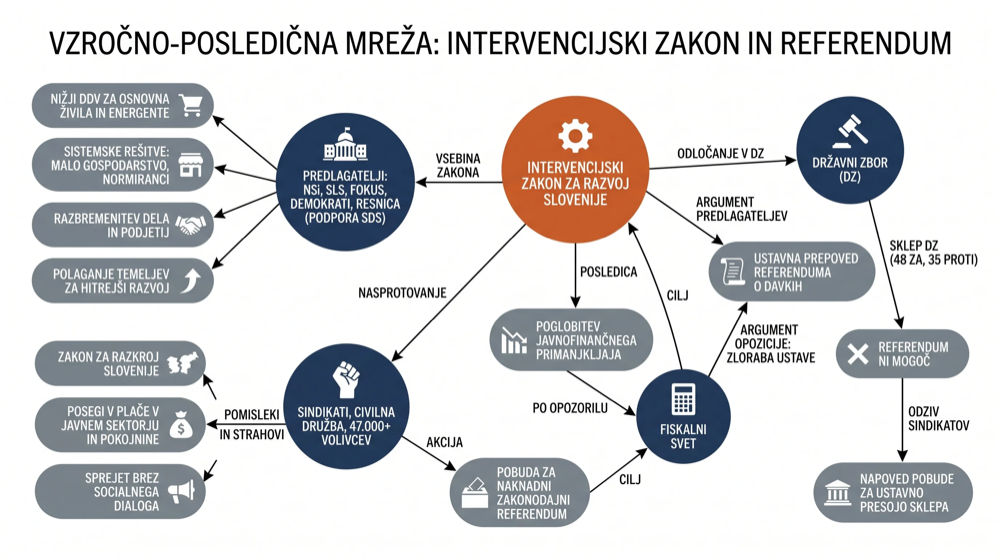
\includegraphics[width=\linewidth]{figs/hero_direct.png}
    \caption{Direct (text$\rightarrow$image)}
  \end{subfigure}\hfill
  \begin{subfigure}{0.42\textwidth}\centering
    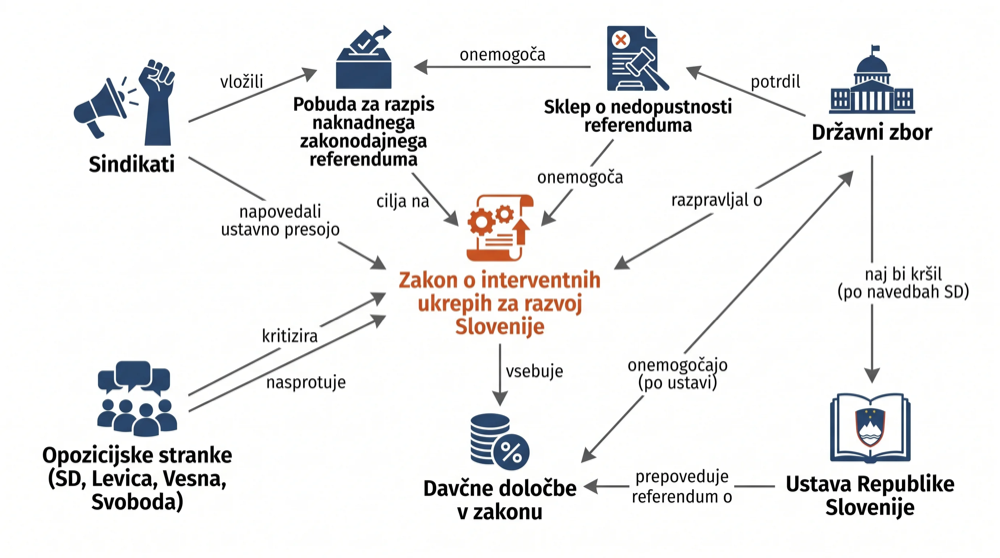
\includegraphics[width=\linewidth]{figs/hero_triplet.png}
    \caption{Triplet$\rightarrow$image}
  \end{subfigure}
  \caption{Hero event (\emph{Intervention-law referendum}, slv-125182). The triplets are sound and the triplet$\rightarrow$image (b) tied the direct image (a) on faithfulness, but the model mis-connected four of its twelve edges---``good triplets, wrong renders.'' The direct image is denser and more polished.}
  \label{fig:hero}
\end{figure*}

\section{Discussion}
The result reframes the contribution. Inserting a triplet stage did not produce a better infographic, and on a black-box basis the direct baseline wins. But the decomposition turns a single, unverifiable image into an \emph{auditable chain}: we can state that extraction is $\sim$70\% clean (with $\sim$5\% hard errors) and, separately, that the rendering stage mis-draws $\sim$19\% of edges---predominantly wrong connections. The black-box pipeline conflates these two error sources; the explicit graph pulls them apart, showing that the single largest avoidable failure lies in generative rendering, not extraction. This is the Semantic-Web payoff in miniature: an explicit, standardizable intermediate enables verification and control that an end-to-end model forecloses.

\textbf{What the explicit intermediate unlocks.} Beyond auditing, materializing the graph enables capabilities the black box cannot (all future work): \emph{selective rendering}---over-extract, then draw only a chosen subgraph (by confidence, salience, or query) instead of letting the model silently omit; \emph{cross-event bridging}---link events through shared entities/triplets, surfacing connections invisible when each event is a separate image; \emph{linking to sentiment}---join graph entities to the system's existing per-publisher sentiment module, attaching ``who covered this, and how'' to each node; and \emph{interactive images}---OCR the rendered nodes so a reader can click one to retrieve its cross-source coverage, sentiment, and omissions.

\section{Limitations and Future Work}
The evaluation is a single rater over a small sample (10 events, 115 triplets), and several rubric axes are subjective. Crucially, only a handful of prompt iterations preceded freezing the prompts; the render and faithfulness results characterize \emph{this} pipeline instance, not an upper bound, and are plausibly improvable with further prompt engineering (e.g.\ structuring the graph input differently for the image model). The triplet schema's node ontology is narrower than free generation, which explains part of the density gap. Future work: gold-standard triplets and a second rater for inter-rater agreement; representing attribution with RDF-star reification~\cite{rdfstar} rather than predicate hedges; normalizing free-text predicates to a controlled vocabulary and aligning entities to an ontology such as Wikidata~\cite{chepurova2025wikontic}; comparing extraction and image models; and improving the deterministic renderer toward icon-level richness so it can rival the generative path on legibility while retaining fidelity.

\section{Conclusion}
Making the hidden knowledge graph of a news infographic explicit does not, by itself, make the picture better---but it makes the pipeline honest. We can see where it succeeds (extraction) and where it fails (generative rendering), and choose a faithful renderer when we must. For a Semantic-Web view of generative pipelines, that inspectability is the point.

\printbibliography

\end{document}
